\documentclass[11pt,a4paper]{article}

% ---------------------------------------------------------------- packages
\usepackage[T1]{fontenc}
\usepackage[utf8]{inputenc}
\usepackage{mathptmx}
\usepackage[scaled=0.92]{helvet}
\usepackage{courier}
\usepackage[hmargin=1in,vmargin=2.3cm]{geometry}
\usepackage{amsmath,amssymb,amsthm}
\usepackage[expansion=false]{microtype}
\usepackage{graphicx}
\usepackage{booktabs,tabularx,multirow,threeparttable}
\usepackage{caption}
\usepackage{float}
\usepackage{enumitem}
\usepackage{xcolor}
\usepackage{tikz}
\usetikzlibrary{arrows.meta,positioning,calc}
\usepackage[numbers,sort&compress]{natbib}
\usepackage{xurl}
\usepackage[hidelinks]{hyperref}
\usepackage[capitalise,nameinlink]{cleveref}

\captionsetup{font=small,labelfont=bf}
\setlist{itemsep=2pt,topsep=4pt}
\setlength{\parskip}{1pt}
\renewcommand{\arraystretch}{1.12}
\setlength{\textfloatsep}{10pt plus 2pt minus 2pt}
\setlength{\intextsep}{8pt plus 2pt minus 2pt}
\setlength{\bibsep}{2pt plus 1pt}
\renewcommand{\bibfont}{\small}

% ---------------------------------------------------------------- notation
\newcommand{\Te}{T_{e}}
\newcommand{\Ta}{T_{a}}
\newcommand{\Th}{T_{h}}
\newcommand{\PTA}{P_{\mathrm{TA}}}
\newcommand{\sTA}{s_{\mathrm{TA}}}
\newcommand{\Zp}{\mathbb{Z}_p^{*}}
\newcommand{\concat}{\,\|\,}
\newtheorem{proposition}{Proposition}
\newcommand{\Fone}{\mathcal{F}_1}
\newcommand{\Ftwo}{\mathcal{F}_2}
\newcommand{\code}[1]{\texttt{#1}}
% provenance of a claim: Paper / Reproduced / Ours / Implementation / Experiment
\newcommand{\prov}[1]{\textsc{\small[#1]}}

\definecolor{ink}{HTML}{14202E}
\definecolor{kgc}{HTML}{6B3FA0}
\definecolor{sen}{HTML}{1D5EA8}
\definecolor{agg}{HTML}{B26A00}
\definecolor{ver}{HTML}{455A6E}

\hypersetup{pdftitle={Reproducing, Auditing and Extending a Certificate-Based Aggregate Signature Scheme for IIoT}}

\begin{document}

% ---------------------------------------------------------------- title page
\begin{titlepage}
\centering
\vspace*{2.2cm}
{\LARGE\bfseries Reproducing, Auditing and Extending a\\[4pt]
Certificate-Based Aggregate Signature Scheme\\[4pt]
for the Industrial Internet of Things\par}
\vspace{1.2cm}
{\large Project Report\par}
\vspace{0.4cm}
{\normalsize A study of: Z.~Qiao \emph{et al.}, ``An Efficient Certificate-Based Aggregate Signature
Scheme With Provable Security for Industrial Internet of Things,''\\
\emph{IEEE Systems Journal}, vol.~17, no.~1, pp.~72--82, 2023.\par}
\vspace{2.2cm}
\begin{tabular}{l@{\hspace{2.5em}}l}
Anurag Kaushal & Roll No.\ 2025202013\\
Pranav Vyas & Roll No.\ 2025202015\\
Md Taufique Hussain & Roll No.\ 2025202007\\
\end{tabular}\par
\vspace{1.2cm}
{\small Code, tests and recorded results:\\[2pt]
\url{https://github.com/Anurag-1205/Certificate-Based-Aggregate-Signature}\par}
\vfill
{\large Research in Information Security\par}
{International Institute of Information Technology, Hyderabad\par}
\vspace{0.6cm}
{Date of submission: November 17, 2026\par}
\vspace*{1cm}
\end{titlepage}

% ---------------------------------------------------------------- abstract
\begin{abstract}
\noindent Qiao \emph{et al.} (IEEE Systems Journal, 2023) show that the certificate-based aggregate
signature (CBAS) scheme of Verma \emph{et al.} can be forged by a malicious key generation centre (KGC),
and propose a repaired scheme that they prove secure and present as costing the same as the scheme it
replaces. We implemented both schemes over two independent elliptic-curve libraries (Ristretto255 via
libsodium and NIST P-256 via OpenSSL), reproduced the paper's forgery, and then tested the repair and
its claims. Our main results are: (i)~the paper's attack works against Verma's scheme in 8 of 8 trials
and fails against the repair, and a controlled ablation shows that binding the nonce commitment $T_i$
into the hash is what stops it; (ii)~Verma's scheme, as the paper describes it, admits a much simpler
key-only universal forgery that needs no observed signature, contradicting the paper's own security
table, and a $2\times2$ ablation shows that each of the repair's two hash bindings closes a different
attack; (iii)~the cost the paper prints for its own scheme is about half the cost of its own
verification equation ($\times1.99$ at $n=100$), and best-effort optimisation of both schemes leaves the
measured gap at about $\times2.4$ rather than closing it; (iv)~in deployment, one invalid signature
silently invalidates an aggregate, a repeated signing nonce reveals every signer secret (three
signatures for an outsider, two for the KGC), and the paper's ``replay resistance'' and ``perfect
forward security'' claims do not hold. All results are produced by running code: 424 tests on both
libraries, two live demonstrations, and an audit script that recomputes every reported number.

\medskip\noindent\textbf{Keywords:} certificate-based signatures, aggregate signatures, Industrial
Internet of Things, malicious KGC, cryptanalysis, reproducibility, nonce reuse.
\end{abstract}

\section{Introduction}\label{sec:intro}

In an Industrial Internet of Things (IIoT) deployment, thousands of sensors report readings that drive
physical processes: temperatures, pressures, valve states. A forged reading can open a valve or shut
down a production line, so every reading must be authenticated. Two engineering pressures shape how
this is done. First, the sensors are constrained and the network is shared, so the verifier should not
have to receive and check $n$ separate signatures; \emph{aggregate signatures}~\cite{boneh2003} let an
aggregator compress $n$ signatures into one object that the cloud checks with a single accept-or-reject
decision. Second, the key infrastructure should be light: a conventional PKI needs certificate storage,
distribution and revocation, while identity-based signatures~\cite{shamir1984} let the key authority
compute every user's private key (\emph{key escrow}). \emph{Certificate-based} cryptography~\cite{gentry2003}
sits between the two: each sensor generates its own key pair, a key generation centre (KGC) issues it a
certificate, and signing needs both, so neither the sensor's key nor the KGC alone suffices to sign.

That design goal only holds if the KGC cannot forge. The KGC holds a master secret key, and master keys
leak: the paper we study cites an incident in which an insider at South Africa's Postbank took a data
centre's master key and stole 3.2 million US dollars~\cite{qiao2023}. A certificate-based aggregate
signature (CBAS) scheme for IIoT must therefore remain unforgeable even against a \emph{malicious} KGC.

\paragraph{The paper under study.}
Qiao \emph{et al.}~\cite{qiao2023} (IEEE Systems Journal, 2023) examine the CBAS scheme of Verma
\emph{et al.}~\cite{verma2020} (CB-CAS, 2020). They show that a malicious KGC that has observed one valid
signature can forge signatures on arbitrary messages, and they propose a repaired scheme. They prove the
repair existentially unforgeable under the discrete-logarithm assumption in the random-oracle model, and
their cost tables present it as exactly as cheap as Verma's scheme.

\paragraph{Our questions.}
We set out to check the paper's claims independently and then to test the repaired scheme further:
\begin{enumerate}[label=\textbf{RQ\arabic*}]
\item Does the paper's attack work, and which change in the repair stops it?
\item Is the repaired scheme as cheap as the paper's tables state, and does a good implementation change
      the answer?
\item Is the paper's attack the weakest attack on Verma's scheme, and which of the repair's changes closes
      which attack?
\item What happens when the repaired scheme is deployed: with a faulty or malicious sensor in a batch,
      with a weak random-number generator, and against the extra security properties the paper claims?
\end{enumerate}

\paragraph{Contributions.}
We distinguish throughout between what the paper claims \prov{Paper}, what we re-ran \prov{Reproduced},
what we measured \prov{Experiment}, our design choices \prov{Implementation}, and results that are new to
this project \prov{Ours}. Known techniques that we only apply to this scheme are named as such.
\begin{enumerate}
\item An implementation of both schemes, faithful to the paper, over two independent prime-order
      groups, with domain-separated hashes, unambiguous encodings and instrumented operation counting, checked by 424
      tests that run on both groups (\cref{sec:method}). \prov{Implementation}
\item Reproduction of the paper's malicious-KGC forgery (8/8 trials) and of the repair's resistance to it
      (0/8), plus a controlled ablation showing that hashing the nonce commitment $T_i$ is the change that
      stops this attack (\cref{sec:repro}). \prov{Reproduced}, ablation \prov{Ours}
\item An audit of the paper's cost tables: the row given for the repaired scheme is identical to Verma's
      row, but its own verification equation costs $(2n+2)\Te+3n\Ta+3n\Th$, about twice the printed value
      ($\times1.99$ at $n=100$), confirmed by timing on two curves and two machines (\cref{sec:cost}).
      \prov{Ours}
\item A key-only universal forgery on Verma's scheme as described in the paper, which needs no observed
      signature and contradicts the paper's Table~II, and a $2\times2$ ablation showing that each of the
      repair's two hash bindings closes a different attack (\cref{sec:keyonly}). \prov{Ours}
\item A best-effort optimisation study showing that a better implementation does not close the cost gap:
      about $\times2.4$ before and after (\cref{sec:opt}). \prov{Experiment}
\item A deployment analysis: the cost of handling invalid signatures at the aggregator
      (\cref{sec:agg}), key recovery from a repeated signing nonce with a hedged-nonce fix
      (\cref{sec:nonce}), and tests of the paper's replay-resistance and forward-security claims
      (\cref{sec:claims}). \prov{Ours}, applying known techniques where stated.
\end{enumerate}

\paragraph{Organisation.}
\Cref{sec:background} gives the background and related work, \cref{sec:schemes} the two schemes, and
\cref{sec:method} our implementation and methodology. \Cref{sec:repro,sec:cost} cover the reproduction and
the cost audit; \cref{sec:keyonly,sec:opt,sec:agg,sec:nonce,sec:claims} the new investigations.
\Cref{sec:discussion} discusses what the results do and do not show, and \cref{sec:conclusion}
concludes. The code, tests, recorded measurements and the commands that reproduce every result are in
the project repository listed on the title page.

\section{Background and Related Work}\label{sec:background}

\subsection{Key infrastructures and certificate-based signatures}
Three ways of binding a public key to an identity frame this work. In a \emph{public-key infrastructure}
a certification authority signs each user's key; verifiers must obtain, store and check certificates and
learn about revocations. In \emph{identity-based} cryptography~\cite{shamir1984} the public key is the
identity itself and a trusted authority derives every private key, so the authority can sign on anyone's
behalf. \emph{Certificateless} cryptography~\cite{alriyami2003} splits the private key between a
user-chosen secret and a partial key from the authority. \emph{Certificate-based}
cryptography~\cite{gentry2003} keeps a user-generated key pair but makes the authority's certificate a
required secret input to signing, so certificates need no separate distribution channel and the
authority cannot sign alone. The schemes studied here are certificate-based.

\subsection{Aggregate signatures}
An aggregate signature scheme~\cite{boneh2003} lets $n$ signatures by $n$ signers on $n$ messages be
combined into one aggregate that verifies only if every component is valid. The motivation in IIoT is
communication and decision cost: the cloud receives one aggregate and makes one accept-or-reject
decision. The aggregate offers no way to tell which component was invalid when verification fails, which
is the starting point of \cref{sec:agg}; identifying bad signatures inside a batch is a studied problem in
batch verification~\cite{pastuszak2000}.

\subsection{Security model}
The paper uses the standard notion of existential unforgeability under adaptive chosen-message attack
(EUF-CMA)~\cite{gmr1988}, with two adversaries specific to certificate-based schemes~\cite{qiao2023}:
\begin{itemize}
\item $\Fone$, a \emph{malicious user}: may replace the public key of any user and obtain keys,
      certificates and signatures, but never holds the master key or the challenge identity's certificate.
\item $\Ftwo$, a \emph{malicious KGC}: holds the master key and hence every certificate, but never the
      challenge identity's secret key, and cannot replace public keys.
\end{itemize}
A scheme is secure if neither adversary can produce a valid signature on a message it did not have
signed. The paper proves its repair secure against both by the forking lemma~\cite{pointcheval2000}. We do
not audit that proof.

To compare attacks we use the taxonomy of Goldwasser, Micali and Rivest~\cite{gmr1988}. A
\emph{key-only attack} sees only public keys; a \emph{chosen-message attack} may also obtain signatures.
A \emph{universal forgery} produces a valid signature on any message the attacker chooses. Key-only
universal forgery is the strongest break: the least access and the most damaging result.

\subsection{Schnorr-type signatures and the commitment in the hash}
Both schemes are Schnorr-like~\cite{schnorr1991}: the signer commits to a fresh nonce $t$ with $T=tP$,
derives a challenge by hashing, and responds with a scalar linear in its secrets. The challenge must hash
the commitment together with the message, $c=H(T,m)$. If it hashes only the message, $c=H(m)$, then $T$
can be chosen \emph{after} $c$ is known, and any response verifies for a suitably solved $T$. This is the
mechanism behind both the paper's attack and our key-only forgery. The nonce must also never repeat: two
Schnorr signatures under one nonce reveal the secret key, which is why modern variants derive the nonce
deterministically from the key and message~\cite{rfc6979,rfc8032}.

\subsection{Forward security}
A forward-secure signature scheme~\cite{bellare1999} divides time into periods and updates the secret key
at each period through a one-way function, erasing the old key, so that a key stolen in period $j$
cannot sign for any earlier period. The paper itself cites a scheme titled as a forward-secure certificate-based signature
scheme~\cite{li2015}. ``Perfect forward secrecy'' is the corresponding property of key exchange, where
session keys remain safe after a long-term key leaks; it does not describe a signature scheme.

\subsection{Cost models}
Papers in this line compare schemes by counting group operations: $\Te$ for a scalar multiplication,
$\Ta$ for a point addition and $\Th$ for a hash to a scalar, priced with measured unit costs. The paper's
Table~IV gives $\Te=0.112$, $\Ta=0.005$ and $\Th=0.004$~ms (and $1.365$~ms for a pairing, which neither
scheme uses)~\cite{qiao2023}. We use these counts and costs to check the paper's tables
(\cref{sec:cost}), and measure real time separately.

\section{The Schemes Under Study}\label{sec:schemes}

\subsection{System model}
\Cref{fig:arch} shows the four parties and six algorithms common to both schemes~\cite{qiao2023}. The
KGC runs \textsf{Setup} once and publishes the system parameters. Each sensor generates its own key pair
(\textsf{KeyGen}) and obtains a certificate from the KGC (\textsf{CertGen}). Sensors sign their readings
(\textsf{Sign}); an aggregator in the plant combines $n$ signatures (\textsf{AggSign}); the cloud server
checks the aggregate with one equation (\textsf{AggVerify}) and either accepts all $n$ readings or rejects
the batch.

\begin{figure}[ht]
\centering
\begin{tikzpicture}[scale=1.2, transform shape,
  party/.style={draw=#1, line width=0.9pt, fill=#1!8, rounded corners=3pt, align=center,
                minimum height=1.05cm, font=\small},
  lab/.style={font=\footnotesize, align=center},
  >={Stealth[length=2.2mm]}]
\node[party=kgc, minimum width=3.4cm] (kgc) at (5.2,3.2) {\textbf{KGC}\\ holds $\sTA$ \\ \textsf{Setup}, \textsf{CertGen}};
\node[party=sen, minimum width=2.4cm] (s1) at (0,1.2) {\textbf{Sensor} $i$\\ \textsf{KeyGen}, \textsf{Sign}};
\node[party=sen, minimum width=2.4cm] (s2) at (0,-0.4) {\textbf{Sensor} $j$\\ \textsf{KeyGen}, \textsf{Sign}};
\node[font=\small] at (0,-1.35) {$\vdots$};
\node[party=agg, minimum width=2.7cm] (agg) at (5.2,0.4) {\textbf{Aggregator}\\ \textsf{AggSign}};
\node[party=ver, minimum width=2.9cm] (cloud) at (10.2,0.4) {\textbf{Cloud server}\\ \textsf{AggVerify}};
\draw[->, kgc, line width=0.8pt] (kgc.west) -| node[lab, above, pos=0.25] {$\mathit{Cert}_i$} (s1.north);
\draw[->, sen, line width=0.8pt] ([xshift=0.6cm]s1.north) |- node[lab, below, pos=0.75] {$pk_i$} ([yshift=-0.3cm]kgc.west);
\draw[->, kgc, line width=0.8pt] (kgc.east) -| node[lab, above, pos=0.3] {public parameters} (cloud.north);
\draw[->, sen, line width=0.8pt] (s1.east) -- node[lab, above, sloped] {$m_i,\ \delta_i$} (agg.west);
\draw[->, sen, line width=0.8pt] (s2.east) -- (agg.west);
\draw[->, agg, line width=1.1pt] (agg.east) -- node[lab, above] {$m_1,\dots,m_n,\ \delta$} (cloud.west);
\node[lab, ver] at (10.2,-0.75) {accept all $n$ or reject};
\end{tikzpicture}
\caption{System model shared by both schemes. In the repaired scheme $\mathit{Cert}_i=(c_i,R_i)$,
$\delta_i=(T_i,z_i)$ and the aggregate is $\delta=(T_1,\dots,T_n,z)$.}
\label{fig:arch}
\end{figure}

\Cref{tab:notation} lists the notation, which follows the paper.

\begin{table}[ht]
\centering\small
\caption{Notation.}\label{tab:notation}
\begin{tabularx}{\linewidth}{lX}
\toprule
Symbol & Meaning \\
\midrule
$G$, $p$, $P$ & a cyclic group of prime order $p$ with generator $P$ \\
$\sTA$, $\PTA=\sTA P$ & KGC master secret key and public key \\
$id_i$, $sk_i$, $pk_i=sk_iP$ & identity, secret key and public key of sensor $i$ \\
$\mathit{Cert}_i$, $c_i$ & certificate of sensor $i$; $c_i$ is its secret scalar part \\
$R_i$ (or $R_{1i}$) & certificate commitment, a public point \\
$T_i=t_iP$ ($R_i$ in Verma) & per-signature nonce commitment; $t_i$ is the nonce \\
$H_0,H_1,H_2$ & hash functions to $\Zp$, modelled as independent random oracles \\
$h_0^i, v_i, u_i$ & the hash values used in certificates and signatures \\
$\Delta$ & public ``state information'' fixed in \textsf{Setup} \\
$\Te,\Ta,\Th$ & cost of a scalar multiplication, a point addition, a hash \\
\bottomrule
\end{tabularx}
\end{table}

\subsection{Verma \emph{et al.}'s CB-CAS}
We implement Verma's scheme as the paper reviews it in its Section~IV-A~\cite{qiao2023}; we did not
cross-check Verma's original article~\cite{verma2020}. The KGC picks $\sTA\in\Zp$. Sensor $i$ picks
$sk_i\in\Zp$ and publishes $pk_i=sk_iP$. The certificate is
\begin{equation}
R_{1i}=r_{1i}P,\qquad c_i=r_{1i}+\sTA\,h_0^i,\qquad h_0^i=H_0(id_i\concat pk_i),
\end{equation}
which anyone can check as $c_iP=R_{1i}+h_0^i\PTA$. To sign $m_i$, the sensor picks a nonce $r_{2i}$ and
computes
\begin{equation}\label{eq:verma-sign}
R_i=R_{1i}+r_{2i}P,\qquad v_i=H_1(m_i\concat pk_i\concat id_i\concat\Delta),\qquad
z_i=r_{2i}+c_i+sk_i v_i,
\end{equation}
and outputs $\delta_i=(R_i,z_i)$. The aggregate is $R=\sum R_i$, $z=\sum z_i$, and it verifies if
\begin{equation}\label{eq:verma-verify}
zP=R+\Big(\sum_i h_0^i\Big)\PTA+\sum_i v_i\,pk_i .
\end{equation}
The aggregate has constant size, one point and one scalar for any $n$. Note that the hash $v_i$ depends
on the message but not on the commitment $R_i$.

\subsection{Qiao \emph{et al.}'s repaired scheme}
The repair changes the certificate and the signature~\cite{qiao2023}. The certificate commitment
$R_i=r_iP$ now enters the certificate hash, and $\mathit{Cert}_i=(c_i,R_i)$ with $R_i$ public:
\begin{equation}
c_i=r_i+\sTA\,h_0^i,\qquad h_0^i=H_0(id_i\concat pk_i\concat R_i).
\end{equation}
To sign, the sensor commits to a fresh nonce, $T_i=t_iP$, and computes two hash values over the message
\emph{and both commitments}:
\begin{gather}
v_i=H_1(m_i\concat pk_i\concat R_i\concat id_i\concat T_i\concat\Delta),\qquad
u_i=H_2(m_i\concat pk_i\concat R_i\concat id_i\concat T_i\concat\Delta),\\
z_i=t_i+c_i u_i+sk_i v_i,\qquad \delta_i=(T_i,z_i). \label{eq:qiao-sign}
\end{gather}
The aggregator outputs $\delta=(T_1,\dots,T_n,z)$ with $z=\sum z_i$; only the scalar half compresses. The
verifier recomputes $h_0^i,v_i,u_i$ and accepts if
\begin{equation}\label{eq:qiao-verify}
zP=\sum_i T_i+\sum_i u_iR_i+\Big(\sum_i u_ih_0^i\Big)\PTA+\sum_i v_i\,pk_i .
\end{equation}
Correctness follows by substituting $z_i$, $c_iP=R_i+h_0^i\PTA$ and $pk_i=sk_iP$. Compared with
Verma's scheme, the repair (1)~hashes $R_i$ into $H_0$, $H_1$ and $H_2$; (2)~hashes the nonce commitment
$T_i$ into $H_1$ and $H_2$; and (3)~scales the certificate and the secret key by two independent hash
values $u_i$ and $v_i$. The price is that each $T_i$ must travel to the verifier, so the aggregate grows
with $n$.

\section{Implementation and Methodology}\label{sec:method}

Every result in this report is produced by running code. This section describes the implementation, how
we checked it, and how we measured. The repository's README lists the command behind each result.

\subsection{Implementation}
Both schemes, all six algorithms each, are implemented in Python~3.12 over native group libraries called
through \code{ctypes}. The reference implementation of the repaired scheme (\code{scheme.py}) is a direct
transliteration of the paper's Section~V-A, with the paper's variable names, so it can be read side by
side with the paper. Optimised variants live in separate modules, so the reference keeps measuring the
algorithm the paper describes. Two printed typos in the paper are corrected in the code: \textsf{KeyGen} prints $pk_i=s_i$ for
$pk_i=s_iP$, and the repaired certificate check uses Verma's $R_{1i}$ where $R_i$ is meant.

\paragraph{Two independent group backends.} \prov{Implementation}
The paper's algebra divides by hash values and its proof relies on a group of prime order. Curve25519
(Ed25519)~\cite{bernstein2012} has cofactor 8, so we use Ristretto255~\cite{rfc9496}, a prime-order group
built on it, through libsodium~1.0.18. A second backend implements NIST P-256~\cite{fips186} through
OpenSSL~3.0.13. The two libraries share no code and represent points differently, so every test is also a
differential test: two independent implementations must agree on every signature, verification result
and operation count. P-256 is also the curve most often deployed in industrial stacks.

\paragraph{Hashing and encoding.} \prov{Implementation}
The paper applies $H_1$ and $H_2$ to identical inputs. Instantiating both with the same hash function
would make $u_i=v_i$ and silently remove the repair's third change. Each oracle therefore gets its own
domain-separation tag, and a test asserts $u_i\neq v_i$ on identical input. Hash inputs are encoded with
length prefixes, because plain concatenation of variable-length fields is ambiguous
(\code{"ab"}$\concat$\code{"c"} and \code{"a"}$\concat$\code{"bc"} collide). Each hash is SHA-512 over the
tagged encoding, reduced modulo the group order from 64 bytes, which makes the bias negligible.

\paragraph{Operation counting.}
Every scalar multiplication, point addition and hash passes through one counting wrapper, so the
$\Te$/$\Ta$/$\Th$ counts of \cref{sec:cost} are measured, not derived by hand. The same instrument
reproduces Verma's published cost rows exactly, which validates the method.

\subsection{Testing}
The test suite has 424 tests: 199 that run once per backend (398) and 26 that need no group, such as the
curve-fitting and aggregator-model tests. A standalone self-test checks 62 algebraic properties of the two
backends before anything else runs. The tests cover round-trip correctness for both schemes up to
$n=17$, rejection of every kind of tampering, the forgeries and their failures, both ablations, the
operation counts, the optimised verifiers against the reference, the aggregator policies, nonce-reuse
recovery and the hedged-nonce fix.

\subsection{Measurement methodology}
Timings are taken on an AMD Ryzen~5 7520U laptop, with a second machine (an Intel Xeon at 2.2~GHz on
Kaggle) used to confirm the timing results. A first sweep on the laptop produced a spurious result,
$n=100$ appearing cheaper than $n=50$, because the CPU clock roughly doubled partway through the sweep.
Two measures address this. A stabilisation step runs real scalar multiplications until the per-operation
cost has stayed constant for several consecutive chunks and at least four seconds have passed. Every
measurement then interleaves all workloads, across both schemes and all values of $n$, takes the median
of several rounds, and calibrates repetitions so that each sample lasts at least 20~ms.

We report \emph{ratios} of per-signer cost, obtained as the slope of a linear fit of aggregate
verification time against $n$ ($n=50$ to $500$), rather than absolute times. Absolute times include Python
and \code{ctypes} overhead and depend on the curve, which is not the paper's: the paper's unit costs come
from a pairing library and it does not name its curve. A ratio between two schemes on the same machine,
curve and library is the quantity the paper's tables make a claim about.

\subsection{Evidence discipline}
Every number in this report and in the accompanying slides is recomputed by one audit script, which
reruns the attacks, counts and tests and reads the recorded benchmark files, asserts each claim, and
stops if any fails. Deterministic results are reported as ``$k/8$'': 4 target messages on each of the 2
backends. These trials confirm that the code behaves as the algebra predicts on both libraries; they are
not statistical samples.

\section{Reproducing the Paper's Attack and Testing the Repair}\label{sec:repro}

\subsection{The malicious-KGC forgery on Verma's scheme}\label{sec:repro-attack}
\prov{Paper}, reproduced. The attacker is the paper's $\Ftwo$, a malicious KGC. It issued sensor $i$'s
certificate $(R_{1i},c_i)$ and has observed one valid signature $(R_i,z_i)$ on a message $m_i$. It does
not know $sk_i$ or the nonce $r_{2i}$, and it wants a signature on a new message $m'$.

From \cref{eq:verma-sign}, the KGC can strip its own contributions: $R_i-R_{1i}=r_{2i}P$, and
$z_i-c_i=r_{2i}+sk_iv_i$, a single scalar that mixes the two unknowns. The weakness is that the hash
$v_i=H_1(m_i\concat pk_i\concat id_i\concat\Delta)$ does not depend on the nonce, so for any new message
the coefficient $v'=H_1(m'\concat pk_i\concat id_i\concat\Delta)$ can be computed in advance. Rescaling by
$\lambda=v'/v_i$ gives
\begin{equation}\label{eq:rescale}
R'=R_{1i}+\lambda\,(R_i-R_{1i}),\qquad z'=c_i+\lambda\,(z_i-c_i),
\end{equation}
which is a valid signature on $m'$ with the unknown nonce $\lambda r_{2i}$: substituting into
\cref{eq:verma-verify} gives $z'P=R'+h_0^i\PTA+v'pk_i$. The attacker never learns $r_{2i}$ or $sk_i$; it
rescales a value it cannot open. Our function \code{forge\_verma} follows the paper's derivation step by
step and takes no secret key as an argument, which a test checks.

\subsection{Results}
We ran the attack for 4 target messages on each backend, against Verma's scheme and, with the same
strategy, against the repaired scheme (\cref{tab:repro}). Against Verma's scheme every forgery verifies,
also inside an aggregate next to an honest signature. Against the repair the rescaling has no fixed
target: the new commitment $T'$ must be chosen before $v'$ can be computed, but the attack defines $T'$
in terms of $v'$. Iterating this circular definition for 16 rounds produced 16 distinct candidates in
every trial and no forgery.

\begin{table}[ht]
\centering\small
\caption{The paper's attack and our ablation (4 messages $\times$ 2 backends).}\label{tab:repro}
\begin{tabular}{llcl}
\toprule
& Scheme & Forgeries that verify & Status \\
\midrule
A & Verma \emph{et al.} & 8 / 8 & broken, as the paper says \prov{Reproduced} \\
B & Qiao \emph{et al.}, repaired & 0 / 8 & the attack does not apply \prov{Reproduced} \\
C & Qiao without the $T_i$ binding & 8 / 8 & broken again \prov{Ours} \\
\bottomrule
\end{tabular}
\end{table}

\subsection{Which change stops the attack}
The repair changes several things at once (\cref{sec:schemes}), so its resistance alone does not say
which change matters. We built a control: the repaired scheme with exactly one change removed, the
nonce commitment $T_i$ dropped from $H_1$ and $H_2$. Everything else is the real scheme's code: the same
\textsf{Setup}, \textsf{KeyGen}, \textsf{CertGen}, aggregation and verification equation, with $R_i$ still
hashed and $u_i,v_i$ still from separate hash functions. The variant is a working scheme: honest
signatures verify and signatures do not transfer to other messages (8/8). The paper's attack succeeds
against it in 8 of 8 trials (row C).

Binding $T_i$ into the hash is therefore \emph{necessary} to stop this attack, all else held fixed. The
paper states the same design rule in its Section~V-A: the commitment $T_i$ ``should be used to generate
the core element of signature'', otherwise a malicious KGC can forge from a known
signature~\cite{qiao2023}. The ablation tests that rule; it does not show that the other changes are
unnecessary, nor that the repaired scheme is secure, which is the paper's proof. \Cref{sec:keyonly}
returns to the other binding.

\section{Auditing the Cost Claims}\label{sec:cost}

The paper's Tables~II and~III give the repaired scheme exactly the same cost as Verma's scheme, and
its Figs.~3--5 plot those rows; its comparative claim, ``best efficiency'' among secure schemes, rests on
them~\cite{qiao2023}. The repaired verification equation \eqref{eq:qiao-verify}, however, has an extra
per-signer term $u_iR_i$ and an extra hash $H_2$ that Verma's \eqref{eq:verma-verify} does not. We
therefore counted the operations of the paper's own algorithms.

\subsection{Operation counts}\label{sec:cost-counts}
\prov{Ours}. \Cref{tab:counts} compares the printed rows with the counts measured by our instrumented
backend. The counts are identical on both backends and at every $n$ tested. Counted the same way, Verma's
scheme reproduces its printed rows exactly (except \textsf{Sign}, which omits one point addition), so the
method is sound and the discrepancy lies in the rows printed for the repaired scheme.

\begin{table}[ht]
\centering\small
\caption{Cost of the repaired scheme: printed in the paper vs counted from its algorithms.}\label{tab:counts}
\begin{tabular}{lll}
\toprule
Algorithm & Paper (Tables II--III) & Counted \\
\midrule
\textsf{Sign} & $1\Te+1\Th$ & $1\Te+2\Th$ \\
\textsf{Verify} (one signature) & $3\Te+2\Ta+2\Th$ & $4\Te+3\Ta+3\Th$ \\
\textsf{AggSign} & $(n-1)\Ta$ & no group operations ($n-1$ scalar additions) \\
\textsf{AggVerify} & $(n+2)\Te+(n+1)\Ta+2n\Th$ & $(2n+2)\Te+3n\Ta+3n\Th$ \\
\bottomrule
\end{tabular}
\end{table}

The \textsf{AggVerify} row printed for the repaired scheme is exactly Verma's row: one scalar
multiplication per signer where the equation needs two. Under the paper's own unit costs, at $n=100$, the
printed row evaluates to $12.729$~ms and the counted row to $25.324$~ms, a factor of $1.99$;
per signer, $0.125$ against $0.251$~ms. The value $12.729$~ms is exactly the bar the
paper plots for its scheme in Fig.~4, so that figure inherits the error. The paper also contradicts
itself: it charges scheme~[6] of its comparison (Verma \emph{et al.}'s PFCBAS) $(2n+2)\Te+(3n-1)\Ta+3n\Th$,
which at $n=100$ is $25.319$~ms, within one point addition of our count for the repaired scheme. One
row errs in the paper's favour: \textsf{AggSign} adds scalars, not points, so the printed $(n-1)\Ta$
overstates it.


\paragraph{Objections considered.}
(a)~\emph{Caching.} $h_0^i$ depends only on static values, so a verifier with a fixed roster can cache
it, removing $n$ hashes. Verma's $h_0^i$ is equally static, so the same caching lowers both schemes and
the difference remains. Caching the point $R_i+h_0^i\PTA$ per signer also reproduces the paper's printed
single-signature row, but the aggregate cost stays at $(2n+1)\Te$: $24.807$~ms at $n=100$, still
$\times1.95$. (b)~\emph{Algebraic folding.} $\sum u_iR_i+(\sum u_ih_0^i)\PTA=(\sum u_ic_i)P$ would be a
single multiplication, but $c_i$ is the signer's secret, so a verifier cannot use it. (c)~\emph{Multi-scalar
multiplication} is an optimisation, not what the tables count; \cref{sec:opt} examines it. A test pins
each of these arguments.

\subsection{Timing confirms the counts}
\prov{Experiment}. Counts are a model, so we also measured. The per-signer cost ratio of the repaired
scheme to Verma's is the slope ratio of aggregate verification time against $n$. The printed rows imply
a ratio of $1.00$; the counted rows predict about 2. Over 11 recorded runs on two curves and two machines
the measured ratio lies between $1.99$ and $2.48$ (\cref{fig:runs,fig:vsn}); \cref{tab:timing} gives the
medians.

\begin{table}[ht]
\centering\small
\caption{Measured per-signer cost ratio (repaired $\div$ Verma; median of runs), against the prediction
from operation counts priced with measured primitive costs.}\label{tab:timing}
\begin{tabular}{llccc}
\toprule
Machine & Curve / library & Runs & Measured & Predicted \\
\midrule
Ryzen 5 7520U & Ristretto255 / libsodium & 5 (3 used) & 2.153 & 2.143 \\
Ryzen 5 7520U & P-256 / OpenSSL & 5 (3 used) & 2.366 & 1.986 (2.363--2.371$^{\dagger}$) \\
Xeon 2.2\,GHz (Kaggle) & Ristretto255 / libsodium & 1 & 2.123 & 2.129 \\
\bottomrule
\end{tabular}

\smallskip
\footnotesize $^{\dagger}$ With each hash priced as the real call, including its point encodings
(\cref{sec:p256-gap}). Medians use the runs whose linear fit had $r^2\ge0.99$; all 11 runs lie in $1.99$--$2.48$.
\end{table}

\begin{figure}[ht]
\centering
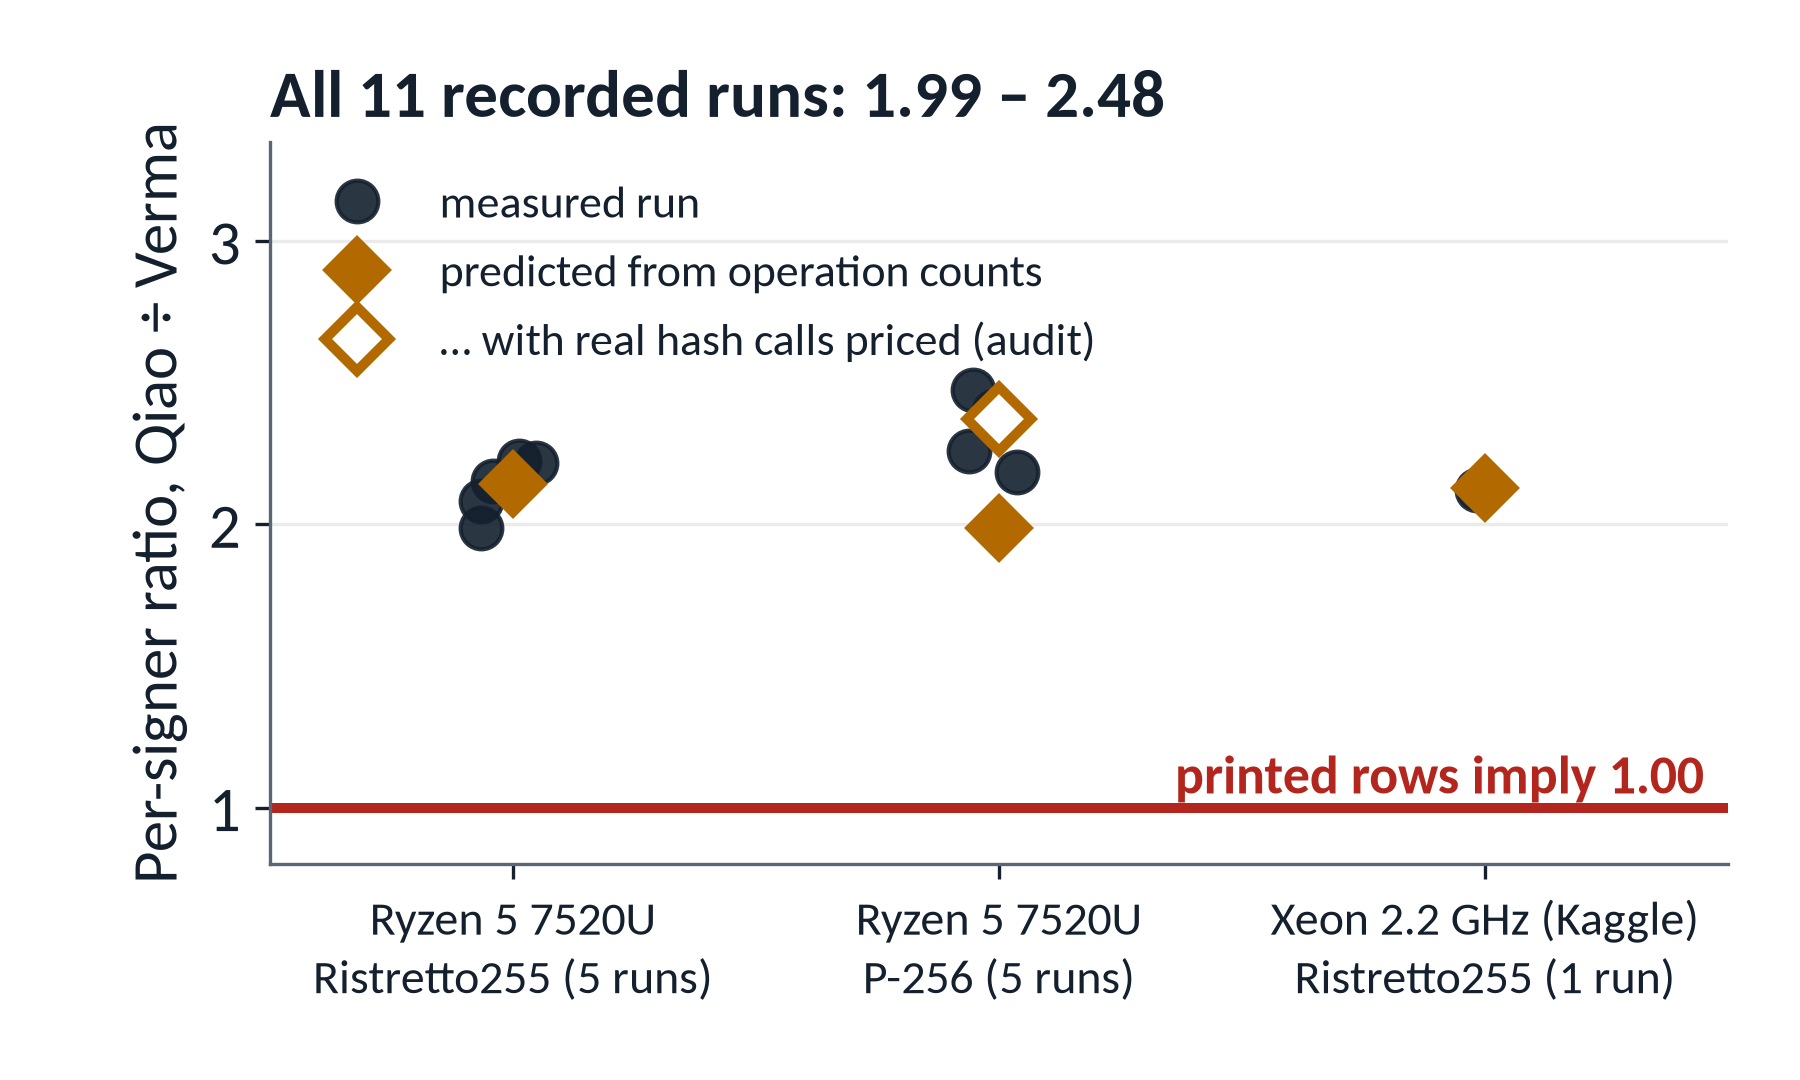
\includegraphics[width=0.74\linewidth]{figures/fig_ratio_runs.png}
\caption{Per-signer cost ratio (repaired $\div$ Verma) in all 11 recorded runs on two curves and two
machines, with the prediction from operation counts. The printed rows imply 1.00. Data:
\nolinkurl{bench/results/sweep_*.json}; the real-hash prediction comes from \code{make hashcost}.}
\label{fig:runs}
\end{figure}

\begin{figure}[ht]
\centering
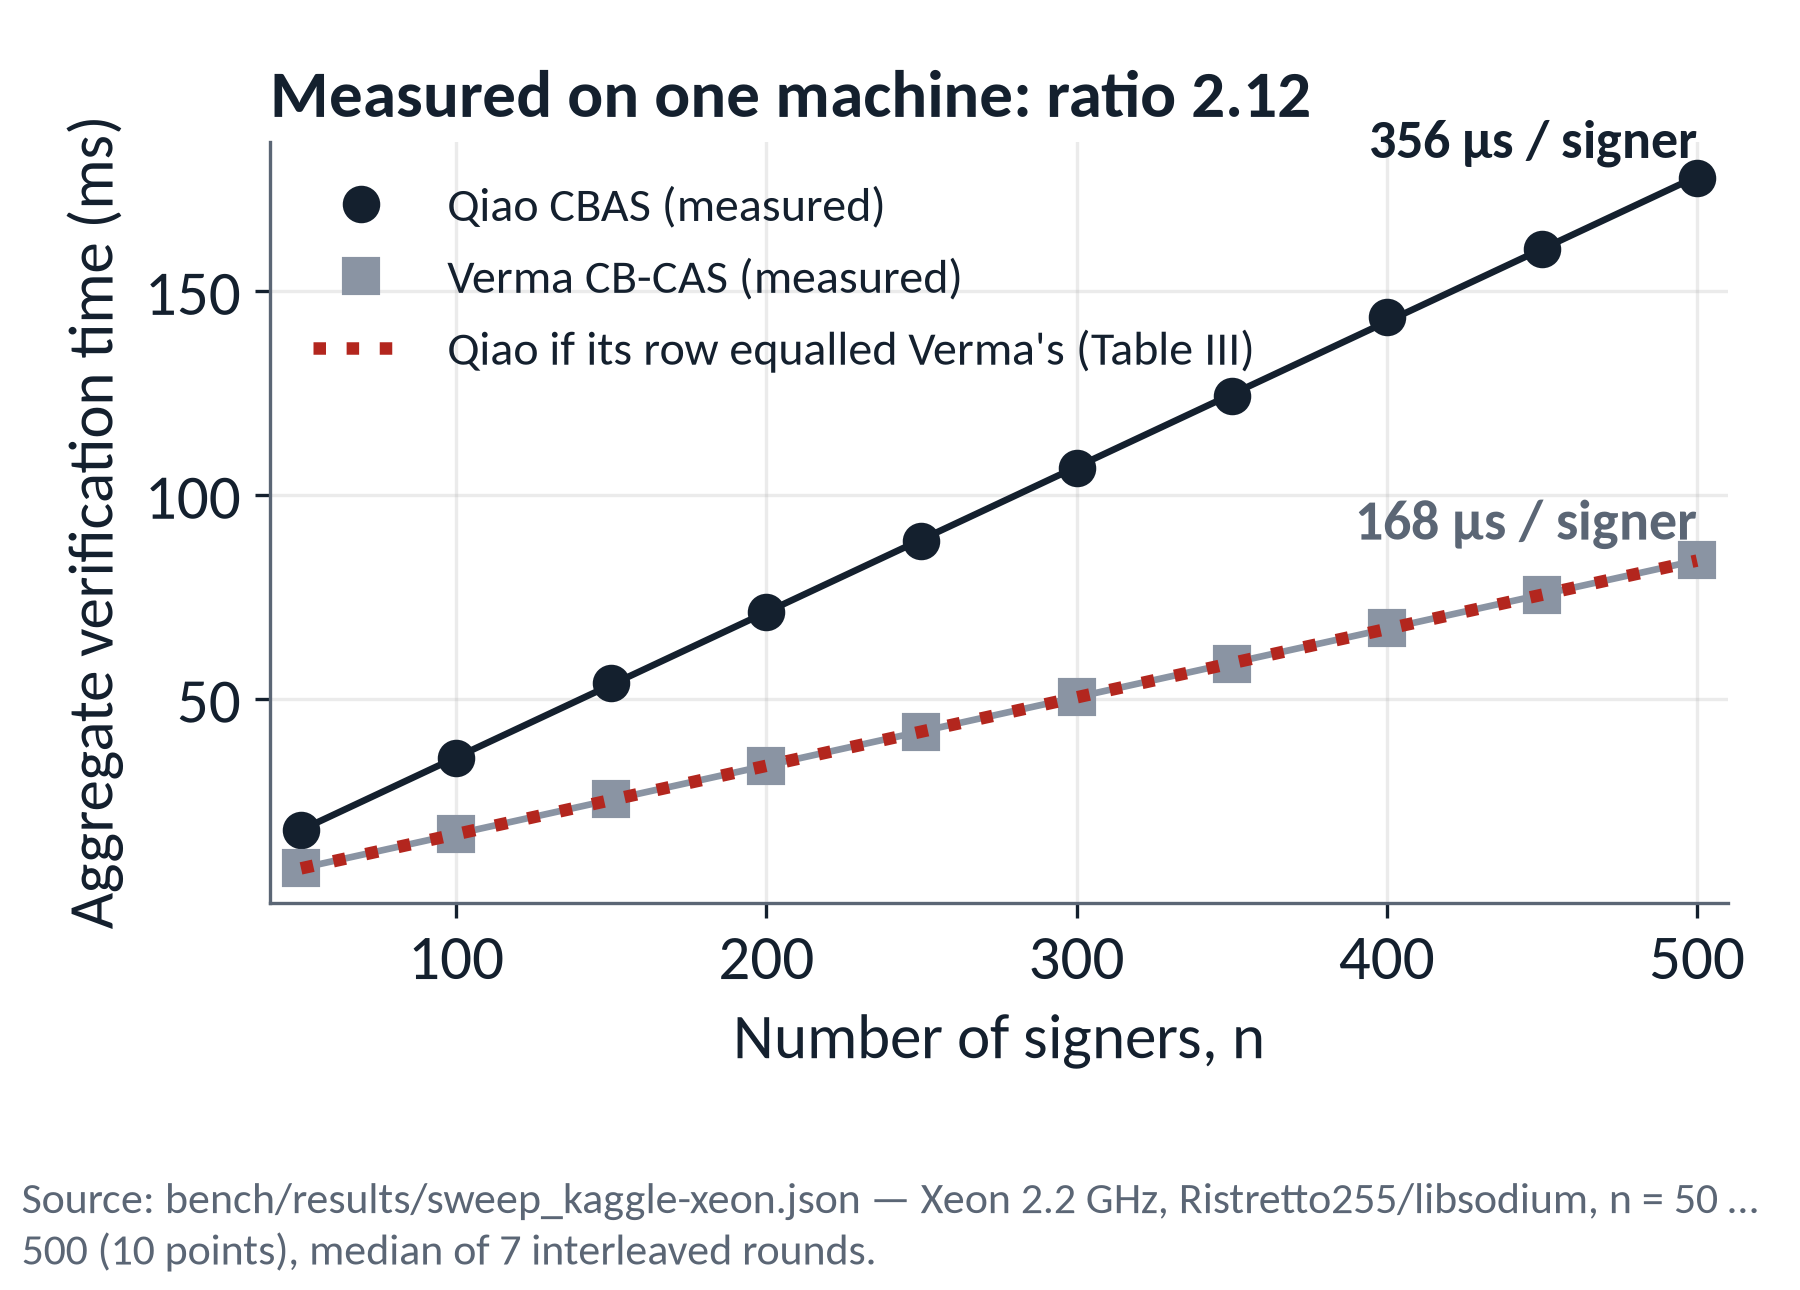
\includegraphics[width=0.74\linewidth]{figures/fig_measured_vs_n.png}
\caption{Aggregate verification time against $n$ on the second machine (Xeon, Ristretto255). The dotted
line is what the repaired scheme would cost if its row equalled Verma's.}
\label{fig:vsn}
\end{figure}

\subsection{Why P-256 timing exceeded the bare count}\label{sec:p256-gap}
On Ristretto255 prediction and measurement agree within $0.5\%$; on P-256 the measured ratio was about
20\% above the bare prediction. The cause is the cost of a real hash call. Each call serialises its point
arguments, and verification of the repaired scheme serialises 8 points per signer ($pk_i$ and $R_i$ in
$H_0$; $pk_i$, $R_i$ and $T_i$ in each of $H_1$ and $H_2$) against Verma's 2; a test counts them. In
OpenSSL a P-256 encoding costs a modular inversion, about twice a point addition, whereas libsodium stores
a Ristretto255 point as its encoding, making the same calls almost free. Pricing the real hash calls
predicts $2.363$--$2.371$ on P-256, against the measured $2.366$. The counts are therefore exact; the bare
model simply prices hashing too cheaply on one library.

\paragraph{Summary.} The paper's own equation costs about twice its printed row. This does not affect
the security of the construction; it affects the paper's efficiency comparison and the figures computed
from the tables.

\section{A Key-Only Universal Forgery}\label{sec:keyonly}

The paper's attacker is strong: a malicious KGC that holds the master key and the victim's certificate and
has observed one signature. We asked whether a much weaker attacker suffices.

\subsection{The forgery}
\prov{Ours}. Consider Verma's verification equation for a single signature,
\begin{equation}\label{eq:verma-single}
zP=R+h_0\PTA+v\,pk,\qquad h_0=H_0(id\concat pk),\qquad v=H_1(m\concat pk\concat id\concat\Delta).
\end{equation}
Neither hash contains $R$, $R$ appears with coefficient 1, and $R$ travels inside the signature, so the
signer (or a forger) chooses it.

\begin{proposition}[Key-only universal forgery]\label{prop:keyonly}
Let $id$ and $pk$ belong to an honestly enrolled signer of Verma's scheme, as specified in Section~IV-A
of~\cite{qiao2023}. Given only the public values $\PTA$, $id$, $pk$ and $\Delta$, an adversary can output,
for any message $m$, a pair $(R,z)$ that the verification equation \eqref{eq:verma-single} accepts. It
succeeds with probability 1, sees no signature, and computes no discrete logarithm.
\end{proposition}

\begin{proof}
The adversary (1) picks any $z\in\Zp$, for example $z=0$; (2) computes $h_0=H_0(id\concat pk)$ and
$v=H_1(m\concat pk\concat id\concat\Delta)$, whose inputs are all public; and (3) sets
$R=zP-h_0\PTA-v\,pk$. The verifier recomputes the same $h_0$ and $v$, because neither depends on $R$, and
\[
R+h_0\PTA+v\,pk=(zP-h_0\PTA-v\,pk)+h_0\PTA+v\,pk=zP,
\]
so \eqref{eq:verma-single} holds. No step can fail, so the probability is 1, and the cost is two hashes,
three scalar multiplications and two point subtractions.
\end{proof}

The forgery uses only point arithmetic: no
secret, no observed signature, no interaction with the KGC or the victim, and no discrete logarithm. In
the taxonomy of~\cite{gmr1988} it is a key-only universal forgery, the strongest kind. It is the familiar
failure of a Schnorr signature whose challenge omits the commitment, $c=H(m)$ instead of
$c=H(R,m)$~\cite{schnorr1991}. We have not found it discussed for Verma's scheme, but we did not survey
the literature exhaustively, so we claim only that the paper does not discuss it.

\paragraph{Results.} Against a real, honestly enrolled victim key, the forgery verifies in 8 of 8 trials
(4 messages $\times$ 2 backends), and 8 of 8 forgeries also pass aggregate verification next to an honest
signature. \Cref{fig:keyonly} shows the captured output of the demonstration.

\begin{figure}[ht]
\centering
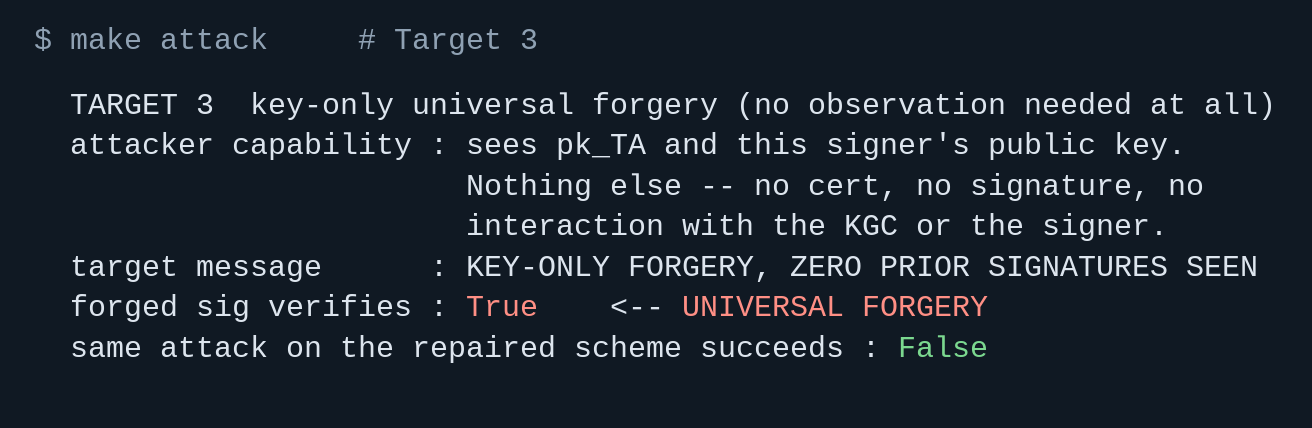
\includegraphics[width=0.9\linewidth]{figures/final_demo1_keyonly.png}
\caption{Captured output of \code{make attack}, Target~3: a forgery from the victim's public key alone
verifies; the same attack on the repaired scheme does not.}\label{fig:keyonly}
\end{figure}

\subsection{It contradicts the paper's Table II}
Table~II of the paper rates Verma's scheme (its reference~[11]) as \emph{secure} against $\Fone$, the
malicious user, and insecure against $\Ftwo$, the malicious KGC~\cite{qiao2023}. The $\Ftwo$ entry is the
paper's own attack (\cref{sec:repro}). The $\Fone$ entry cannot be right: our forger has strictly less
power than $\Fone$, which may additionally replace keys and obtain signatures, so whatever it achieves
$\Fone$ achieves too. This holds for Verma's scheme as the paper specifies it in its Section~IV-A, which
is the scheme the paper's table rates; we did not check Verma's original article~\cite{verma2020}.

\subsection{Why the repaired scheme resists it}
In the repaired equation \eqref{eq:qiao-verify}, $R$ enters all three hashes and $T$ enters two. To solve
for $R$ an attacker needs $h_0$, $u$ and $v$; to compute them it needs $R$. The only route left is a
search for a fixed point of the hash functions: guess $R$, compute the hashes, solve for the $R$ the
equation would require, and compare. In every trial 16 rounds of this search produced 16 distinct
candidates and no forgery. This shows the attack does not apply; it is not a proof of security, which is
the role of the paper's theorem.

\subsection{Which binding closes which door}
The repair binds two commitments at once: $T$ (the signature's nonce commitment) and $R$ (the certificate
commitment). We removed each in turn, keeping everything else, and attacked each variant both by solving
for $T$ and by solving for $R$ (\cref{tab:2x2}).

\begin{table}[ht]
\centering\small
\caption{The $2\times2$ ablation. Each cell reports which attack succeeds (8/8 trials per cell).}
\label{tab:2x2}
\begin{tabularx}{\linewidth}{lXX}
\toprule
& $R$ hashed & $R$ not hashed \\
\midrule
$T$ hashed & \textbf{Repaired scheme}: both attempts fail &
  \textbf{$R$ removed}: solving for $R$ forges, but only under an attacker-chosen $R$ (public-key replacement) \\
$T$ not hashed & \textbf{$T$ removed}: solving for $T$ forges with the victim's real certificate (key-only) &
  \textbf{Verma}: solving for $R$ forges; $R$ travels in the signature (key-only) \\
\bottomrule
\end{tabularx}
\end{table}

In each broken variant the other attempt still fails (8/8), so each binding blocks a different attack
and neither covers for the other. The two open doors differ in kind. $T$ travels in every signature, so
the $T$-removed forgery is a key-only forgery against the real public key. In the repaired scheme, by
contrast, $R$ belongs to the certificate, so the $R$-removed forgery verifies only if the verifier
accepts an attacker-chosen $R$; under the real certificate value it fails in 8 of 8 trials. That is
public-key replacement, the power the paper grants $\Fone$, and it is exactly the reason the paper gives
for hashing $R$. The cell thus confirms the paper's stated rationale with code.

\paragraph{The general rule.} Any value that appears in the verification equation with a known
coefficient but in no hash is a free variable, and an attacker can fix everything else and solve for it.
The paper states this rule for $T_i$ alone, in the context of its one attack; the $2\times2$ shows the
same mechanism for either commitment independently.

\section{Does Optimisation Close the Cost Gap?}\label{sec:opt}

A fair objection to \cref{sec:cost} is that no deployment verifies term by term: a real verifier batches
the work. We therefore optimised both verifiers and asked whether the gap closes.

\subsection{Optimisations}
\prov{Implementation}. Two optimisations are applied to both schemes.
\begin{enumerate}
\item \textbf{Multi-scalar multiplication (MSM).} The whole verification equation is evaluated in one
      native call (OpenSSL's \code{EC\_POINTs\_mul}) instead of one call per term. Sums whose coefficient
      is 1 (the repaired scheme's $\sum T_i$ and Verma's aggregate $R$) are plain point additions outside
      that call.
\item \textbf{A prepared roster.} An industrial fleet is fixed, so each sensor's point encodings and its
      certificate hash $h_0^i$ never change and are computed once per roster, not once per batch. For the
      repaired scheme the roster also caches $C_i=R_i+h_0^i\PTA$, because
      $u_iR_i+u_ih_0^i\PTA=u_iC_i$ folds two multi-scalar terms per signer into one. Verma's $h_0^i$
      already collapse into a single $\PTA$ term, so it has nothing equivalent to fold.
\end{enumerate}
In this best-effort shape the repaired scheme's multi-scalar call has $2n$ full-scalar terms
($u_iC_i$ and $v_ipk_i$) and Verma's has $n+1$ ($v_ipk_i$ and one $\PTA$ term): 1000 against 501 at
$n=500$. A test fixes this shape, so no coefficient-1 term can enter the call. Every optimised path is
checked against the reference implementation on both backends, for valid signatures and for each kind of
tampering.

\subsection{Results}
\prov{Experiment}. \Cref{fig:opt} shows the per-signer cost on P-256 at each stage. As specified, the
repaired scheme costs $169.5$~$\mu$s per signer against Verma's $71.5$ (ratio $2.37$). Fully optimised it
costs $53.7$ against $22.4$ (ratio $2.40$). Both schemes become about three times faster, and the ratio
does not move. Over four runs the ratio was $2.32$--$2.38$ as specified and $2.36$--$2.45$ optimised.

\begin{figure}[ht]
\centering
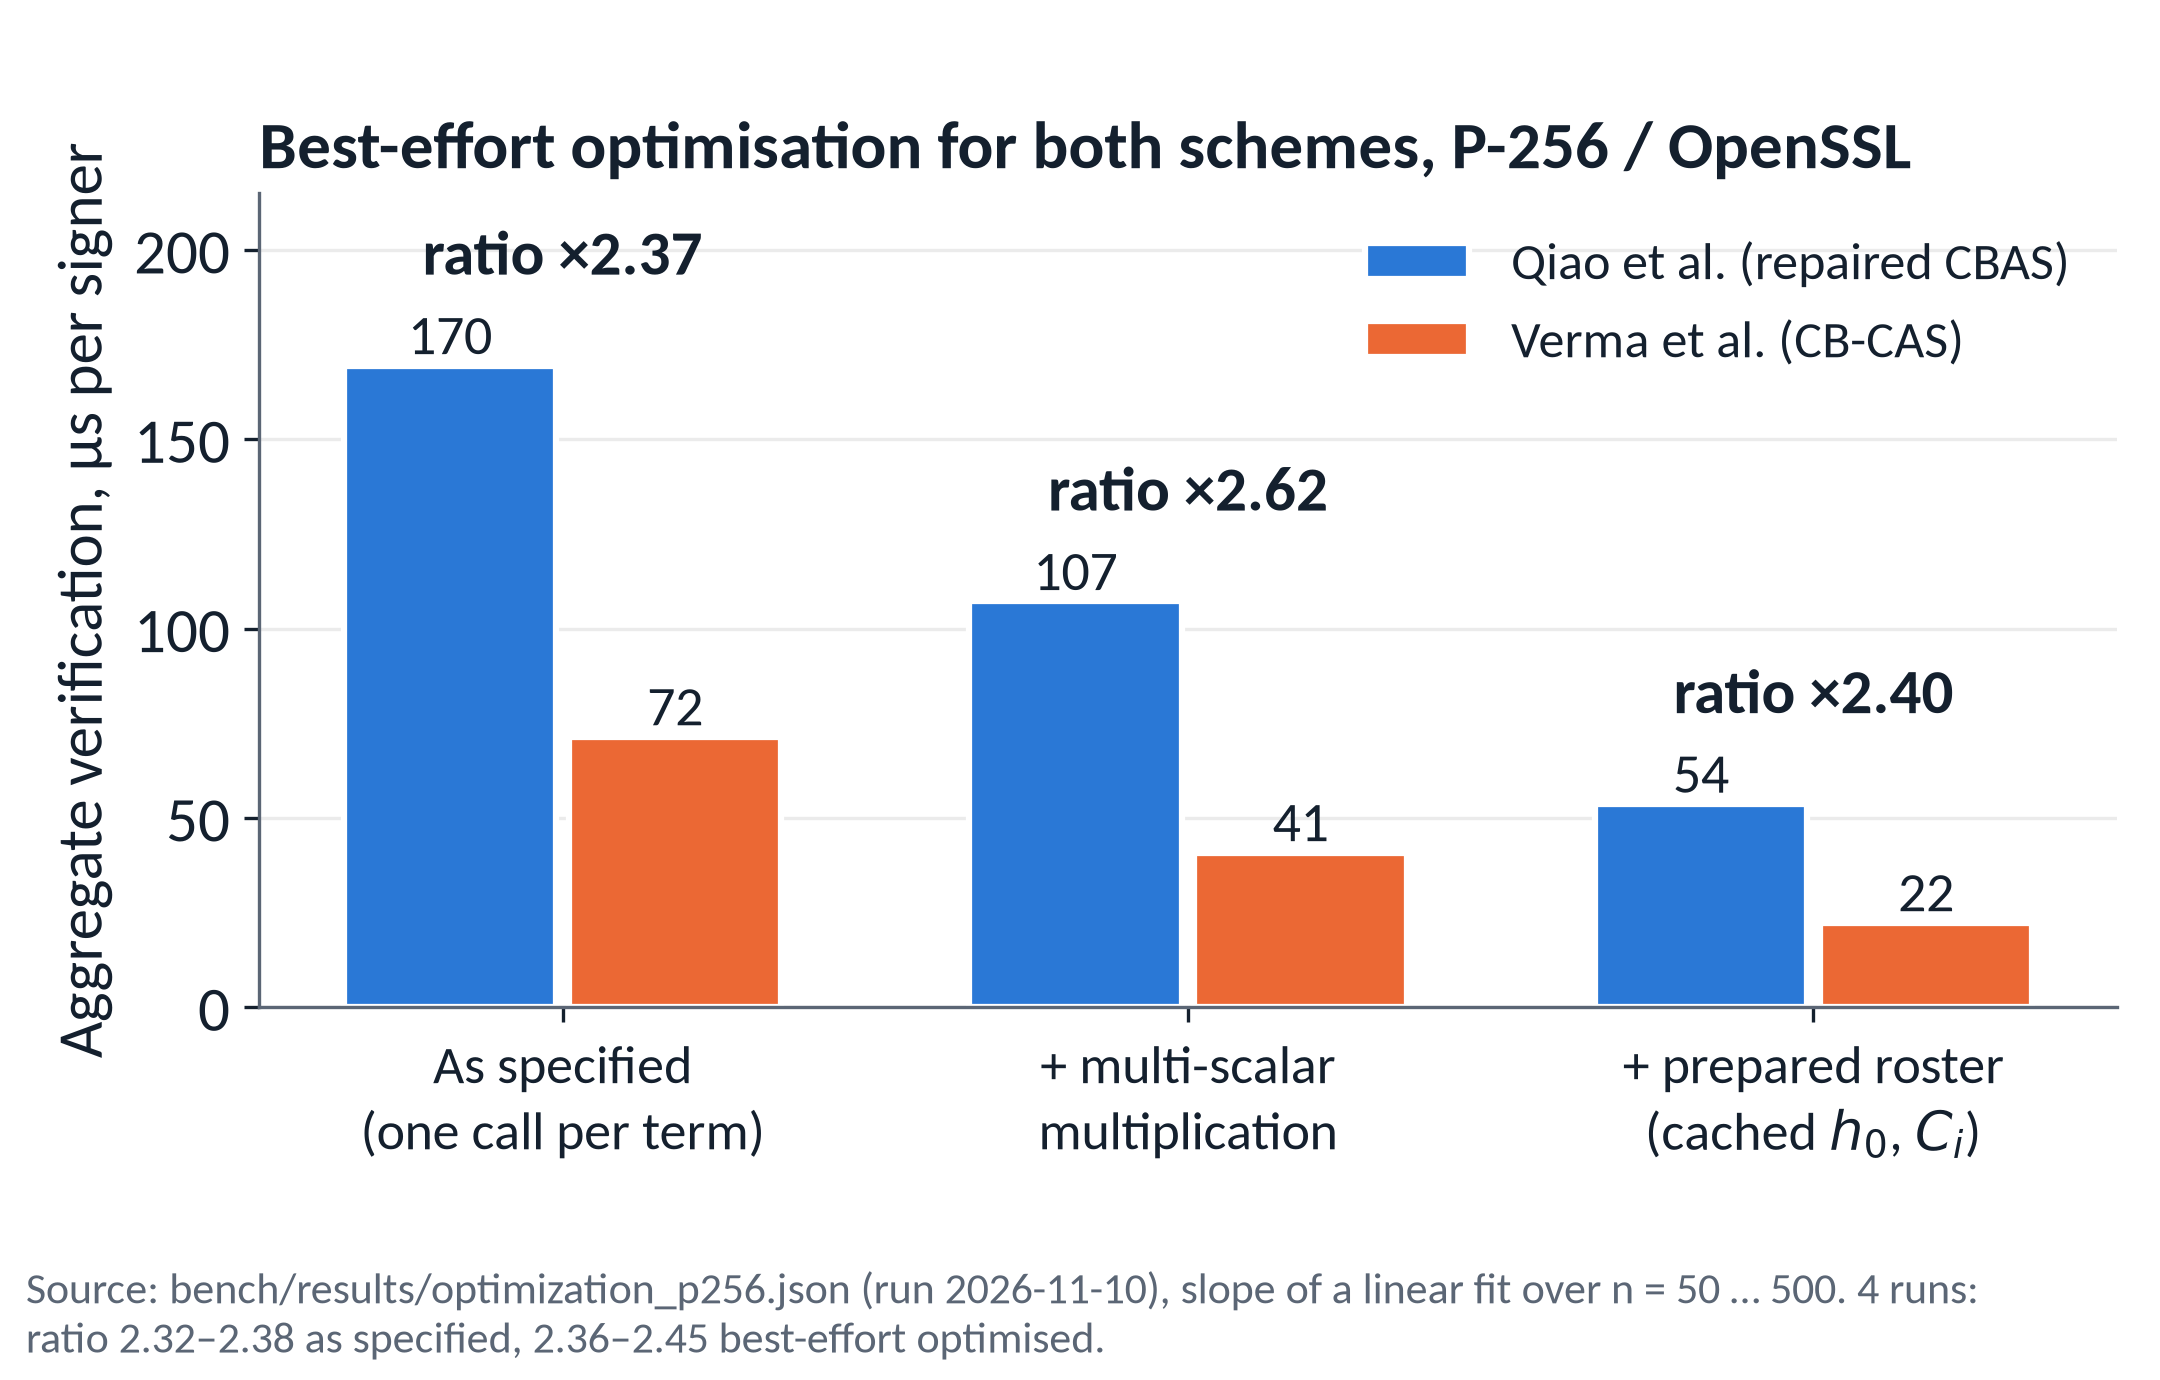
\includegraphics[width=0.85\linewidth]{figures/final_optimisation.png}
\caption{Per-signer aggregate-verification cost on P-256 at each optimisation stage, both schemes in
their best-effort shape. The middle stage is higher for the repaired scheme because it still recomputes
$h_0^i$ and its encodings for every batch.}
\label{fig:opt}
\end{figure}

On Ristretto255 libsodium offers no native multi-scalar routine, so only the roster helps. The ratio
barely moves: $2.02$--$2.20$ as specified and $1.99$--$2.14$ optimised. Which optimisation pays depends on the library rather than the scheme: OpenSSL keeps
points in projective coordinates, so additions are cheap and encoding costs an inversion, while libsodium
keeps a point as its encoding, so encoding is nearly free and additions are expensive.

The ratio stays a little above 2 because the repaired scheme needs two full-scalar terms per signer
against Verma's one, plus one more hash per signer and the $n$ additions for the $T_i$. Either way, the
paper's ratio of $1.00$ is not rescued by a good implementation.

\subsection{Two measurement mistakes, and what they teach}
Equal treatment means giving each scheme its own best-effort implementation, and we got it wrong twice,
once in each direction. Our first version gave the prepared roster to the repaired scheme only and
reported a ratio of $1.63$, which suggested that optimisation closes the gap. Our second version fed the
coefficient-1 $T_i$ into the multi-scalar call as $3n+1$ terms and did not cache $C_i$; it reported about
$3.0$ (between $2.95$ and $3.07$), which suggested the gap \emph{widens}. A review of our own presentation
caught the second error. With both schemes in their best-effort shape the ratio is about $2.4$, the same
as before optimisation. Comparing a careful implementation of one scheme with a careless one of the other
measures the implementations, not the schemes.

\paragraph{Signer side.} On the sensors, which are the constrained devices, caching the static encodings
speeds up \textsf{Sign} on P-256 from $74.8$ to $43.9$~$\mu$s ($1.70\times$) and leaves Ristretto255
unchanged. Group operations stay at $1\Te+2\Th$, and the nonce is still drawn fresh for every signature;
a test checks this, because a cached nonce would leak the keys (\cref{sec:nonce}).

\section{The Aggregator in Practice}\label{sec:agg}

The paper treats the aggregator as harmless: it ``does not use their own private information'' and only
merges signatures~\cite{qiao2023}. That is true, and it is why aggregation does not weaken security. But
merging is a sum, $z=\sum z_i$. If one signature is invalid (a faulty sensor, a corrupted link or an
attacker) the aggregate fails verification, and the sum no longer says which component was wrong. One
bad sensor thereby denies service to every honest sensor in its batch. This is a known property of
aggregation, and locating bad signatures in a batch is a studied problem~\cite{pastuszak2000}; the
paper's system model simply leaves it out. We confirmed it on our implementation (one corrupted signature
in 32 makes the whole aggregate fail), and our contribution is a measurement of what handling it costs.

\subsection{Three aggregator policies}
\prov{Implementation}.
\begin{itemize}
\item \textbf{BLIND} (the paper's model): merge everything. A single bad signature loses the batch and the
      culprit cannot be found.
\item \textbf{PREVERIFY}: verify each signature before merging and drop the bad ones.
\item \textbf{RETAIN}: merge optimistically but keep the individual signatures. If the aggregate fails,
      split the batch in halves and verify each half as an aggregate, recursively. A clean half costs one
      aggregate verification whatever its size, so $f$ faults among $n$ cost on the order of $f\log_2 n$
      verifications. One bad signature among 32 was located with 11 verifications.
\end{itemize}
None of the policies uses secret material, so the paper's security argument is unaffected; a test
inspects the code to confirm this.

\subsection{Which policy, when}
\prov{Experiment}, \prov{Ours}. We simulated batches of $n=200$ signatures on P-256, each signature bad
independently with a given probability, 5 trials per rate, using measured verification costs.
\Cref{tab:agg} reports the total aggregator and cloud work per signature actually delivered.

\begin{table}[ht]
\centering\small
\caption{Cost per delivered signature (ms), P-256, batches of 200, 5 trials per row.}\label{tab:agg}
\begin{tabular}{rrrrrl}
\toprule
Fault rate & Bad per batch & BLIND & PREVERIFY & RETAIN & Cheaper of the two that recover \\
\midrule
0.0\% & 0.0 & 0.0566 & 0.1645 & 0.1163 & RETAIN \\
0.1\% & 0.0 & 0.0566 & 0.1598 & 0.1163 & RETAIN \\
0.5\% & 0.8 & 0.1414 & 0.1612 & 0.2384 & PREVERIFY \\
2.0\% & 3.4 & batch lost & 0.1626 & 0.4058 & PREVERIFY \\
5.0\% & 7.8 & batch lost & 0.1705 & 0.4781 & PREVERIFY \\
10.0\% & 18.4 & batch lost & 0.1784 & 0.5795 & PREVERIFY \\
\bottomrule
\end{tabular}

\smallskip
\footnotesize At the 0.1\% rate no trial drew a bad signature, so the first two rows are both clean batches.
\end{table}

BLIND is cheapest while every batch is clean, but from a 2\% fault rate it delivered nothing in any trial.
RETAIN beats PREVERIFY only on clean batches; from about one bad signature per batch of 200, PREVERIFY is
cheaper, and its cost stays nearly flat up to 10\%. The crossover is low because verifying a signature on
its own costs only $1.7$ times its share of an aggregate verification ($0.098$~ms against $0.057$~ms per
signature), not the order of magnitude one might expect. That makes pre-verification affordable.

\paragraph{Recommendation.} Where sensors almost never fail, RETAIN is cheapest. Where an attacker can
submit bad signatures, the attacker chooses the fault rate, so PREVERIFY is the safe default: it costs
about $2.9$ times a blind aggregation on a clean batch and never loses one. An aggregator too constrained
to verify can still limit the damage by sub-batching: under our measured cost model the best sub-batch
size falls from 25 signatures at a 0.1\% fault rate to 2 at 10\%. This is an availability result, not a weakness in the
cryptography.

\section{Nonce Reuse on Sensors}\label{sec:nonce}

Every signature of the repaired scheme uses a fresh random nonce $t_i$, and the paper only states that
$t_i$ is chosen uniformly at random~\cite{qiao2023}. Sensors are where randomness fails in practice: a
generator stuck or re-seeded after a reboot, a firmware or virtual-machine image cloned together with its
seed, or too little entropy at boot. We asked what a repeated nonce costs.

\subsection{Key recovery}
The attack is the standard nonce-reuse attack on Schnorr-type signatures; our contribution is working it
out for this scheme. From \cref{eq:qiao-sign}, $z_i=t_i+c_iu_i+sk_iv_i$, where $u_i$ and $v_i$ are hashes
of public data. Every signature made under the same nonce $t$ is one more linear equation in the same
unknowns, and the repetition is visible because the same commitment $T=tP$ appears in each signature.

How many signatures are needed depends on the scheme and the attacker (\cref{tab:nonce}). In Verma's
scheme the certificate term $c_i$ has coefficient 1, so the nonce and the certificate merge into one
unknown and two signatures reveal $sk_i$ (although Verma's scheme is forgeable with none,
\cref{sec:keyonly}). The repair multiplies $c_i$ by the per-message hash $u_i$, which makes it a separate
unknown: an outsider needs three signatures and solves a $3\times3$ linear system for $t$, $c_i$ and $sk_i$
(\cref{app:nonce}). With only two signatures, every guess of $sk_i$ fits some $c_i$, and picking the right
one is as hard as a discrete logarithm. The KGC, however, issued the certificate and already knows $c_i$,
so two signatures give it $sk_i$, the very key that certificate-based signatures promise the KGC never
learns.

\begin{table}[ht]
\centering\small
\caption{Signatures under one nonce needed to recover the signer's secrets (8 trials each).}\label{tab:nonce}
\begin{tabular}{llcl}
\toprule
Scheme and attacker & Unknowns & Signatures & Result \\
\midrule
Verma, anyone & $sk_i$ and $r_{2i}+c_i$ (merged) & 2 & secret key recovered, 8/8 \\
Repaired, outsider & $t$, $c_i$, $sk_i$ & 3 & both secrets recovered, 8/8 \\
Repaired, the KGC & $t$, $sk_i$ (knows $c_i$) & 2 & $sk_i$ recovered, 8/8 \\
Repaired, hedged nonce & no shared nonce & --- & attack cannot start, 8/8 \\
\bottomrule
\end{tabular}
\end{table}

The recovered keys are checked against $pk_i$ and the certificate equation before use. With them the
attacker signs a message of its choice with a fresh nonce; the forgery verifies (8/8) and passes
aggregate verification next to honest signatures (8/8). The server sees only valid signatures throughout
(\cref{fig:nonce}).

\begin{figure}[ht]
\centering
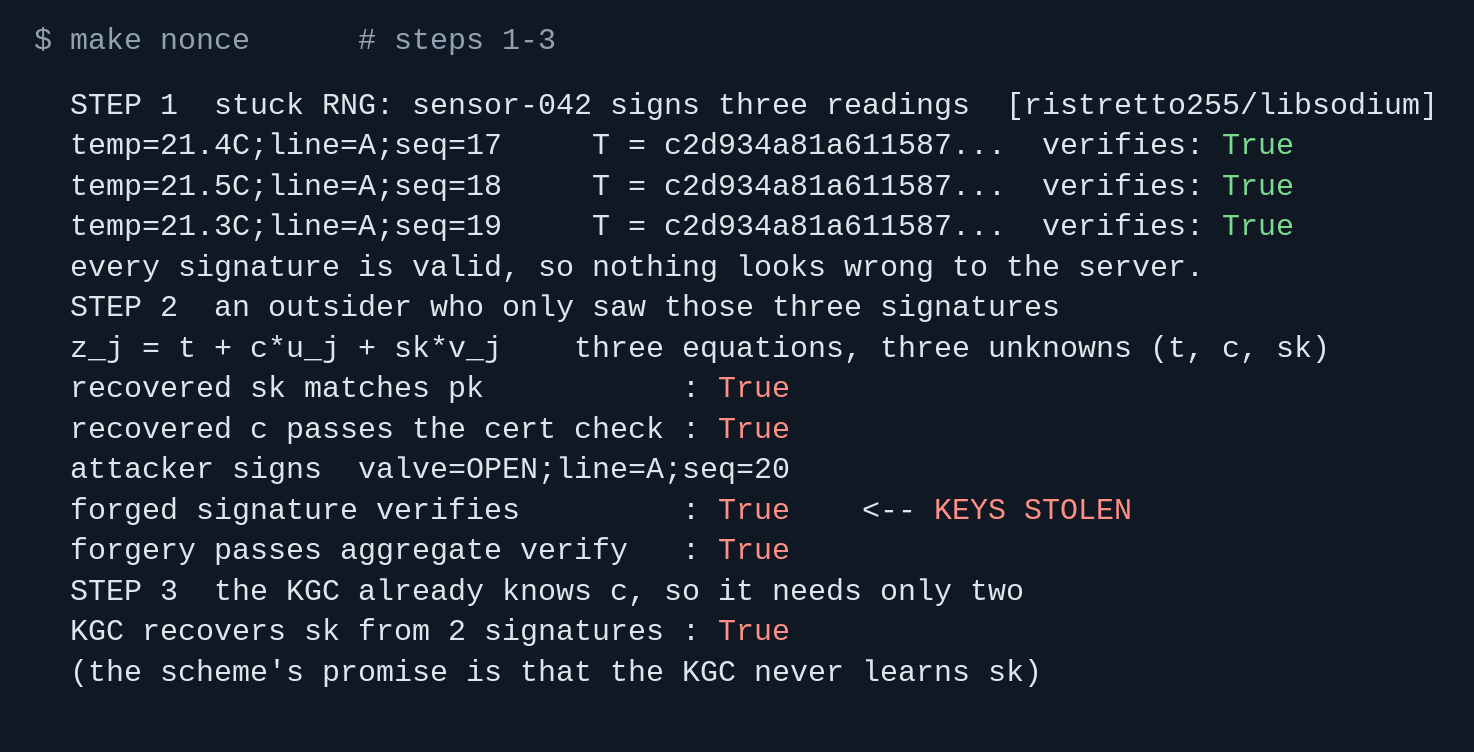
\includegraphics[width=0.9\linewidth]{figures/final_demo2_attack.png}
\caption{Captured output of \code{make nonce}: three readings signed under a stuck generator share one
$T$ and all verify; an outsider recovers both secrets and signs \code{valve=OPEN}; the KGC needs only two
signatures.}\label{fig:nonce}
\end{figure}

\subsection{The fix: a hedged nonce}
\prov{Implementation}, using a standard technique~\cite{rfc6979,rfc8032}. Instead of taking the nonce
straight from the generator, the signer derives it from its secrets and the message and mixes in the
generator's output:
\begin{equation}
t_i=H_{\mathrm{nonce}}(sk_i,\ c_i,\ m_i,\ pk_i,\ R_i,\ id_i,\ \Delta,\ \text{fresh randomness}).
\end{equation}
The secrets keep the nonce unpredictable, the message makes different messages get different nonces even
when the generator is stuck, and the fresh randomness keeps a working generator useful against fault
attacks on purely deterministic nonces. The signing equation and the signature format are unchanged, so
every existing verifier accepts hedged signatures, also in aggregates mixed with ordinary ones. With the
generator stuck, the three nonces were distinct in 8 of 8 trials, all signatures verified, and the
recovery attack could not start. The paper specifies no nonce derivation at all.

\section{The Paper's Additional Security Claims}\label{sec:claims}

Beyond the proven unforgeability, the paper's Section~V-C lists four further security properties. Two are
testable and we tested them.

\subsection{``Resist replay attacks''}
The paper's argument, in full: ``The signature algorithm of our CBAS scheme is probabilistic, so the
different random values will be used every time the algorithm is run, and the different signature will
be obtained even the same message takes as the input.''~\cite{qiao2023}

Signing is indeed randomised. It does not follow that replays are resisted: a replay attack does not sign
anything, it re-sends an old valid message and signature, and that pair still verifies. On both backends
an old signature verified again, and it also verified inside a new aggregate, even when the same signature
appeared twice in one batch (2/2 each). The paper sets $\Delta$ once in \textsf{Setup} and never says it
changes; if a deployment rotated $\Delta$ per epoch, old signatures would stop verifying in the next epoch,
but replays within an epoch would still succeed. Replay protection needs freshness that the verifier
checks, such as a sequence number or timestamp in the message, or rejection of repeated $T_i$. Replay is a
protocol-level property; randomised signing does not provide it. \textbf{The claim does not hold as
argued.}

\subsection{``Perfect forward security''}
The paper's argument, in full: ``In our scheme, no one can obtain the random value that used to created
the signature, hence, our proposal provides perfect forward security.''~\cite{qiao2023}

The paper gives no definition and no proof. For signatures, forward security has a standard
meaning~\cite{bellare1999}: secret keys evolve through time periods, so a key stolen later cannot sign for
an earlier period. The repaired scheme has no time periods and no key update; $sk_i$ and $\mathit{Cert}_i$
are fixed for life. We tested the consequence: keys recovered while the system was in epoch~1 (through the
nonce reuse of \cref{sec:nonce}) signed a back-dated epoch-0 reading that verified, also inside an
aggregate with a genuine epoch-0 signature (2/2). The argument's premise also fails: ``no one can obtain the
random value'' assumes a perfect generator, and with a repeated nonce $t$ is recovered exactly. Nonce
secrecy is needed for unforgeability; it does not give forward security. The paper itself cites a scheme
titled as forward-secure and certificate-based~\cite{li2015}, so the notion was available to the authors.
\textbf{The claim is not supported}; making it true would need a key-evolving construction, not a change
of wording.

\section{Discussion}\label{sec:discussion}

\subsection{Summary of findings}
\Cref{tab:findings} lists every result with its provenance and evidence. One reproduces the paper; the
others are ours, either audits of the paper's claims, measurements, or new analysis. Where a known
technique is applied to this scheme (nonce reuse, hedged nonces, bad-signature identification), only the
application is claimed.

\begin{table}[ht]
\centering\small
\caption{All results, with provenance and evidence.}\label{tab:findings}
\begin{tabularx}{\linewidth}{>{\raggedright\arraybackslash}X>{\raggedright\arraybackslash}p{2.7cm}>{\raggedright\arraybackslash}p{4.1cm}}
\toprule
Result & Kind & Evidence \\
\midrule
The paper's malicious-KGC attack forges Verma signatures & Reproduced & 8/8 \\
The repair stops it, and the $T_i$ binding is the change that does & Reproduced + ablation & 0/8; ablation 8/8 \\
The repaired scheme costs about twice its printed row & Audit & $\times1.99$ at $n=100$; timing 2.12--2.37 \\
Anyone with a public key can forge Verma's scheme; Table II is wrong & Ours & 8/8, 8/8 in aggregate \\
Hashing $T$ and hashing $R$ each block their own attack & Ours & $2\times2$, 8 trials per cell \\
Best-effort optimisation of both schemes does not close the gap & Experiment & $\times2.37\to\times2.40$ \\
Pre-verifying a batch is cheap, so one bad signature need not sink it & Ours (applied) & $1.7\times$ per signature \\
A repeated nonce reveals every secret: 3 signatures, or 2 for the KGC & Ours (applied) & 8/8 \\
The replay and forward-security claims do not hold & Ours & both tested \\
\bottomrule
\end{tabularx}
\end{table}

\subsection{What the paper gets right}
Our findings should not be read as a rejection of the paper. Its diagnosis of Verma's scheme is correct
and reproduces exactly. Its repair resisted every forgery we tried, the paper's own attack and our key-only
attack alike, and both of its hash bindings turn out to be necessary. The aggregator uses no secret
material, which a test confirms; that aggregate security then follows is the paper's argument, which we
did not audit. Nothing we found contradicts the paper's unforgeability theorem. Our findings concern the
efficiency comparison, deployment, and the additional properties claimed in Section~V-C.

\subsection{Threats to validity}
\begin{itemize}
\item \textbf{The proof.} We did not audit the paper's EUF-CMA proof (Theorem~1 and its lemmas). Failed
      attacks are evidence about those attacks only, not about security.
\item \textbf{Verma's scheme.} We implemented it from the paper's description (Section~IV-A), not from
      Verma's original article. Our key-only forgery and the contradiction with Table~II therefore concern
      the scheme as the paper specifies and rates it.
\item \textbf{Timing.} Absolute times include Python and \code{ctypes} overhead, and our curves are not
      the paper's. We therefore report ratios between schemes on the same machine, curve and library,
      supported by exact operation counts that are identical on both libraries. Timings come from a laptop
      and one cloud machine; we did not measure on sensor hardware.
\item \textbf{Simulated faults.} The stuck generator of \cref{sec:nonce} and the faulty signatures of
      \cref{sec:agg} are simulated in software, with independent faults at fixed rates.
\item \textbf{Our own errors.} Twice our optimisation comparison was unequal (\cref{sec:opt}); both errors
      were caught and corrected, and tests now pin the corrected behaviour.
\item \textbf{Novelty.} The mechanism of our key-only forgery is textbook Schnorr hygiene; we did not
      survey the literature exhaustively and claim only that the paper does not discuss it.
\end{itemize}

\section{Conclusion}\label{sec:conclusion}

We reproduced, audited and extended Qiao \emph{et al.}'s certificate-based aggregate signature scheme for
IIoT, with every result produced by running code on two independent elliptic-curve libraries. Three
conclusions stand out.

\begin{enumerate}
\item \textbf{Verma's scheme is broken more simply than the paper says.} Beyond the paper's
      malicious-KGC attack, which we reproduced, anyone holding a public key can forge, contradicting the
      paper's Table~II. The underlying rule, that every commitment in the verification equation must be
      hashed, explains both attacks and both of the repair's hash bindings.
\item \textbf{The repair works, but costs more than printed.} Its own verification equation costs about
      twice the row the paper prints, and about $2.4$ times Verma's in measured time. A best-effort
      optimisation of both schemes does not change that.
\item \textbf{Deploying the repair still needs care.} Pre-verify signatures at the aggregator, derive
      nonces with a hedged construction, and add verifier-checked freshness; the paper's replay-resistance
      and forward-security claims do not hold.
\end{enumerate}

\paragraph{Future work.} Three directions remain open: an audit of the paper's security proof,
measurements on constrained sensor hardware, and a comparison with Verma \emph{et al.}'s original
specification.


\clearpage
\bibliographystyle{unsrtnat}
\bibliography{refs}


\end{document}
